%%%%%%%%%%%%%%%%%%%%%%%%%%%%%%%%%%%%%%%%%
% Short Sectioned Assignment
% LaTeX Template
% Version 1.0 (5/5/12)
%
% This template has been downloaded from:
% http://www.LaTeXTemplates.com
%
% Original author:
% Frits Wenneker (http://www.howtotex.com)
%
% License:
% CC BY-NC-SA 3.0 (http://creativecommons.org/licenses/by-nc-sa/3.0/)
%
%%%%%%%%%%%%%%%%%%%%%%%%%%%%%%%%%%%%%%%%%

%----------------------------------------------------------------------------------------
%	PACKAGES AND OTHER DOCUMENT CONFIGURATIONS
%----------------------------------------------------------------------------------------

\documentclass[paper=a4, fontsize=10pt]{article} % A4 paper and 10pt font size

\usepackage[T1]{fontenc} % Use 8-bit encoding that has 256 glyphs
%\usepackage{fourier} % Use the Adobe Utopia font for the document - comment this line to return to the LaTeX default
\usepackage[english]{babel} % English language/hyphenation
\usepackage{amsmath,amsfonts,amsthm} % Math packages

\usepackage{lipsum} % Used for inserting dummy 'Lorem ipsum' text into the template
\usepackage{courier}
\usepackage{sectsty} % Allows customizing section commands
\setlength{\columnsep}{5mm}

\usepackage{geometry}
 \geometry{
 a4paper,
 total={170mm,257mm},
 left=20mm,
 top=20mm,
 }
 
 \usepackage{graphicx}
\graphicspath{ {images/} }

\usepackage{indentfirst}

\setlength\parindent{0pt} % Removes all indentation from paragraphs - comment this line for an assignment with lots of text

%----------------------------------------------------------------------------------------
%	TITLE SECTION
%----------------------------------------------------------------------------------------


\begin{document}


\begin{titlepage}

\newcommand{\HRule}{\rule{\linewidth}{0.5mm}} % Defines a new command for the horizontal lines, change thickness here

\center % Center everything on the page
 
%----------------------------------------------------------------------------------------
%	HEADING SECTIONS
%----------------------------------------------------------------------------------------

\textsc{\LARGE UCD Smurfit Graduate School of Business}\\[1.5cm] % Name of your university/college

\includegraphics[scale = 0.6]{images/logo.png} \\ [1cm]
\textsc{\Large Numerical Analytics and Software}\\[0.5cm] % Major heading such as course name

%----------------------------------------------------------------------------------------
%	TITLE SECTION
%----------------------------------------------------------------------------------------

\HRule \\[0.4cm]
{ \LARGE \bfseries Programming Assignment 2}\\[0.4cm] % Title of your document
\HRule \\[1.5cm]
 
%----------------------------------------------------------------------------------------
%	AUTHOR SECTION
%----------------------------------------------------------------------------------------

\begin{minipage}{0.4\textwidth}
\begin{flushleft} \large
\emph{Authors:}\\
\small{Eoghan \textsc{Aherne}}\\
\small{Louis \textsc{Carnec}}\\
\small{Conor \textsc{Reid}} %(16202630 - MSc B.A Part-time)}\\ % Your name
\end{flushleft}
\end{minipage}
~
\begin{minipage}{0.4\textwidth}
\begin{flushright} \large
\emph{Lecturer:} \\
\small{Dr. Sean \textsc{McGarraghy}} % Supervisor's Name
\end{flushright}
\end{minipage}\\[4cm]

% If you don't want a supervisor, uncomment the two lines below and remove the section above
%\Large \emph{Author:}\\
%John \textsc{Smith}\\[3cm] % Your name

%----------------------------------------------------------------------------------------
%	DATE SECTION
%----------------------------------------------------------------------------------------
\vspace{3cm}
{\large \today}\\[1cm] % Date, change the \today to a set date if you want to be precise

\vfill % Fill the rest of the page with whitespace

\end{titlepage}

%----------------------------------------------------------------------------------------
%	MAIN BODY
%----------------------------------------------------------------------------------------
%\setlength{\parindent}{10ex}
%Context
\tableofcontents
\clearpage
\onecolumn

\section{Overview}

\subsection{Mathematical Issues}

\subsubsection{4.0}
\subsubsection{4.1}

\subsection{Applications}

\subsection{Questions}
useful to check for convergence of the residual to zero?\\
what matrix norms might be useful and why?\\
scaling be helpful?\\
which matrices do you get expect convergence and which do not? why?\\
effect of different values of tolerance?\\
effect of an ill-conditioned matrix?\\

\section{Design}

\subsection{4.0}
\subsection{4.1}

The implementation of the Black-Scholes-Merton pricing problem found in the module \texttt{tridiagM.py} takes advantage of the fact that the Black-Scholes differential equation as a system of linear equations ($\textbf{A}\textbf{f} = \textbf{b}$) can be written as a tridiagonal $(N-1)\times(N-1)$ matrix. This tridiagonal matrix, $\textbf{A}$, which by definition is a sparse matrix, can be solved using the Sparse SOR algorithm
 which solves for vector $\textbf{x}$ the system of linear equations $\textbf{A}\textbf{x} = \textbf{b}$ by successive iteration. 

We are able to approximate all option prices for a given stock price for all $m \in M$ by approximating the previous time step using a system of linear equations. There are two approximation in finding option prices for all time steps $m$. 

The first of these entails approximating put option prices at time $T$ given Stock prices and a known put option strike price, $X$. Using this approximation for $f_{n,M}$, we can solve the system of linear equation for option prices at previous time periods $f_{n,m}$.

Given that the matrix $\textbf{A}$ represents the finite difference constants relating $f_{n, m-1}$ to $f_{n, m-1}$ and that we can approximate the $N$ European put option prices at $f_{n,M}$, where $M=T$ and time at which the option is at maturity, given the fact that the portfolio must 

$P = -f + \frac{\partial{f}}{\partial{S}}S$
$\left( -\sigma S \frac{\partial{f}}{\partial{S}} +\sigma S \frac{\partial{f}}{\partial{S}} \right) dz = 0 $

 
\subsubsection{Creating the Grid}
To solve for option prices at all time steps we need create a grid of stock prices (S, the stock price vector) and of M time steps until the option reaches maturity (T).
Options have expiration dates or maturity. For example, an option expires in 12 days (T=12) and since our time steps is days ($k=T/M=1$) we have that M=12. If our time step was half a day (k=0.5) for the same expiry date in 12 days, the grid would have 24 time steps ($M = 12 \times 0.5$).
Stock prices can be any non-negative real number. However the grid must start at 0 since the put option price is the strike price when the stock price is zero ($f_{0,m} = X$).

A function (\texttt{createSandT}) was created to return two vectors for stock prices and times. 


\subsection{Implementation issues}
\subsection{Design Decisions}

\section{Testing}

\clearpage
\section*{Appendix}

\begin{figure}[h!]
\center
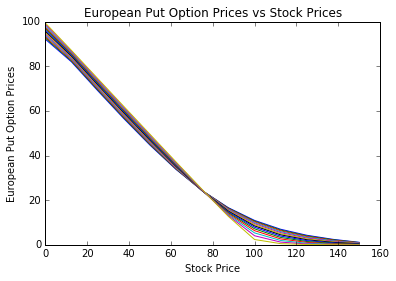
\includegraphics[scale=0.8]{vary1212.png}
\caption{Distribution of put option prices against stock prices for m $T=12$, $M=12$, $k=1$}
\end{figure}

\begin{figure}[h!]
\center
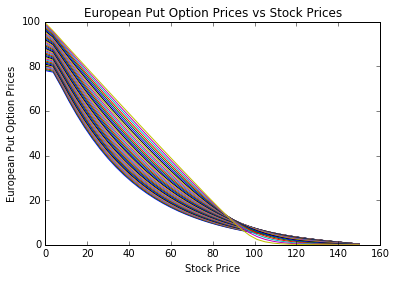
\includegraphics[scale=0.8]{vary1240.png}
\caption{Distribution of put option prices against stock prices for m $T=12$, $M=40$, $k=0.3$}
\end{figure}

\begin{figure}[h!]
\center
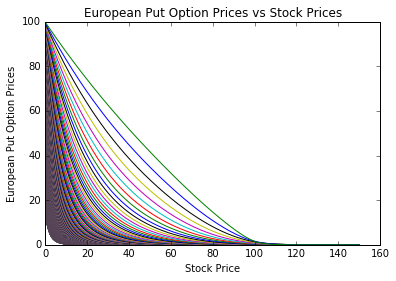
\includegraphics[scale=0.8]{vary12365.png}
\caption{Distribution of put option prices against stock prices for m $T=12$, $M=365$, $k=0.033$}
\end{figure}


\begin{figure}[h!]
\center
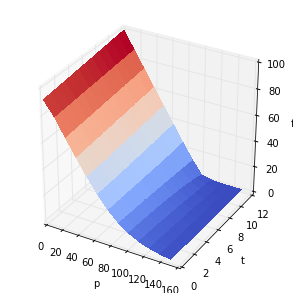
\includegraphics[scale=0.8]{3d_k_12_12.png}
\caption{3D Plot of European Put Option Prices for $T=12$, $M=12$, $k=1$}
\end{figure}

\begin{figure}[h!]
\center
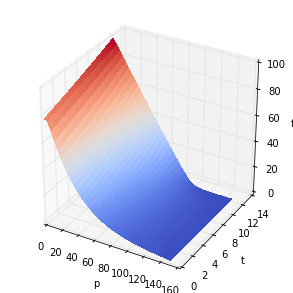
\includegraphics[scale=0.8]{3d_k_12_40.png}
\caption{3D Plot of European Put Option Prices for $T=12$, $M=40$, $k=0.3$}
\end{figure}

\begin{figure}[h!]
\center
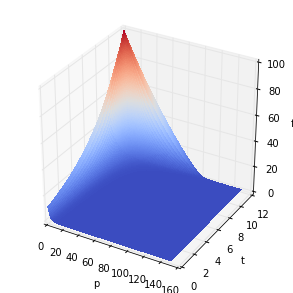
\includegraphics[scale=0.8]{3d_k_12_365.png}
\caption{3D Plot of European Put Option Prices for $T=12$, $M=365$, $k=0.033$}
\end{figure}

\clearpage
\begin{thebibliography}{9}
\bibitem{someitem} 
Some Reference
 
\end{thebibliography}


\end{document}